\chapter*{Proposition 24}
\label{prop:24}

\begin{figure*}[ht]
    \begin{center}
    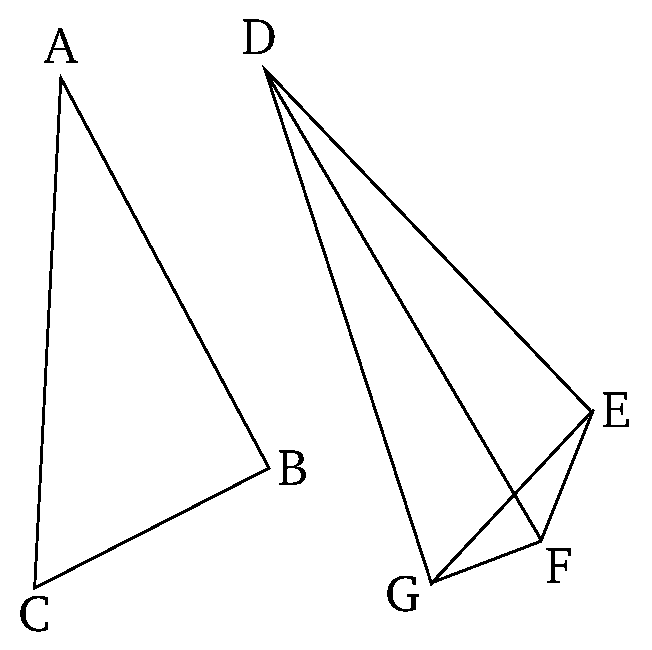
\includegraphics[width=0.5\linewidth]{figures/fig24e.eps}
    \label{fig:prop_24}
    \end{center}
\end{figure*}

If two triangles have two sides equal to two sides, respectively,
but (one) has the angle encompassed by the equal straight-lines greater than the (corresponding)
angle (in the other), then (the former triangle) will also have a base greater than the base (of the latter).

Let  $ABC$ and $DEF$ be two triangles having the two sides $AB$ and $AC$
equal to the two sides $DE$ and $DF$, respectively. (That is), $AB$ (equal) to $DE$, and
$AC$ to $DF$.  Let them also have the angle at $A$ greater than the angle at $D$.
I say that the base $BC$ is also greater than the base $EF$.

For since angle $BAC$ is greater than angle $EDF$, let (angle) $EDG$, equal to
angle $BAC$,  have been constructed at  the point $D$ on the straight-line $DE$ [Prop.~1.23]. And let $DG$ be made equal to either of $AC$ or $DF$ [Prop.~1.3], and let $EG$ and $FG$ have been joined.

Therefore, since $AB$ is equal to $DE$ and $AC$ to $DG$, the two (straight-lines)
$BA$, $AC$ are equal to the two (straight-lines) $ED$, $DG$, respectively.
Also the angle $BAC$ is equal to the angle $EDG$. Thus, the base $BC$ is equal
to the base $EG$ [Prop.~1.4]. Again, since $DF$ is equal to $DG$, angle $DGF$
is also equal to angle $DFG$ [Prop.~1.5]. Thus, $DFG$ (is) greater than $EGF$.
Thus, $EFG$ is much greater than $EGF$. And since triangle $EFG$ has angle $EFG$
greater than $EGF$, and the greater angle is subtended by the greater side [Prop.~1.19], side $EG$ (is) thus also greater than $EF$. But $EG$ (is) equal to
$BC$. Thus, $BC$ (is) also greater than $EF$.

Thus, if two triangles have two sides equal to two sides, respectively,
but (one) has the angle encompassed by the equal straight-lines greater than the 
(corresponding) angle (in the other), then (the former triangle) will also have a base greater than the base (of the latter).
(Which is) the very thing it was required to show.


\section*{Commentary}

Euclid did not cover the case where $D$ and $G$ are on different sides of $EF$ (Fig.~\ref{fig:prop_24b}). Below we augment Euclid's proof to cover this case. The resulting proof is significantly more complicated than Euclid's proof.

\begin{figure*}[ht]
    \begin{center}
    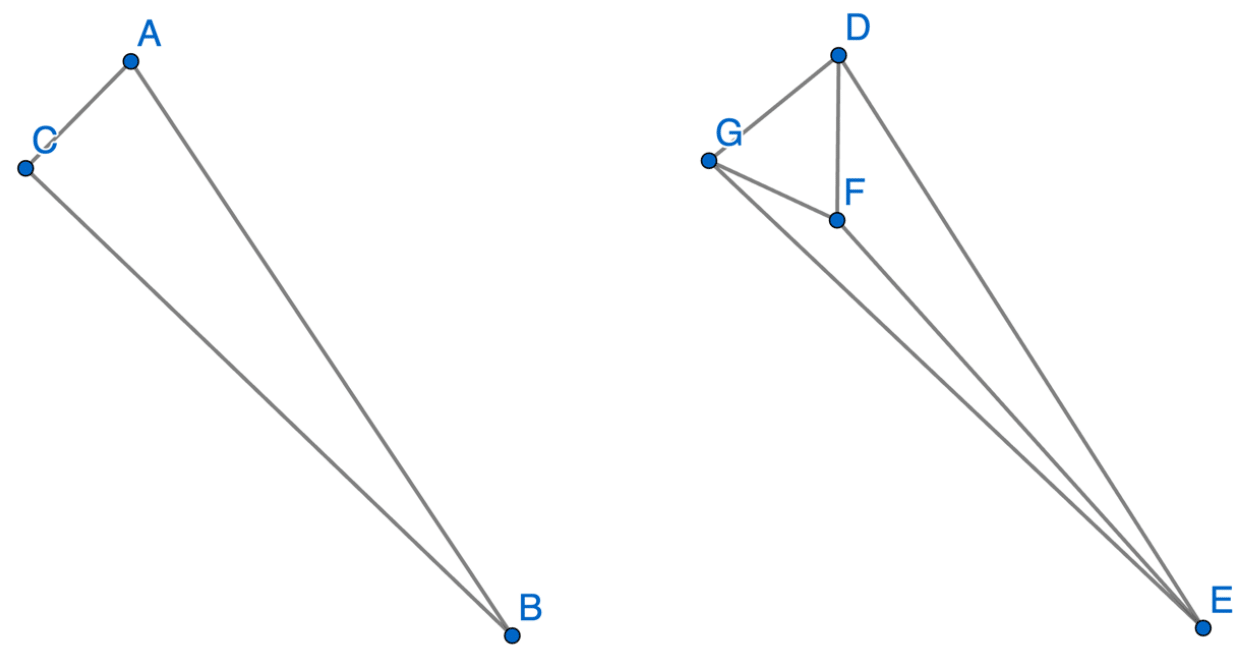
\includegraphics[width=0.35\linewidth]{figures/proposition_24.png}
    \caption{The case in Proposition~24 missed by Euclid.}
    \label{fig:prop_24b}
    \end{center}
\end{figure*}


\begin{proposition}\label{proposition_24}\lean{Elements.Book1.proposition_24}\leanok
    $\triangle~ABC$ and $\triangle~DEF$ are two triangles s.t., $|AB|=|DE|$, $|AC|=|DF|$, and $\angle~BAC~>~\angle~EDF$. Then, $|BC|~>~|EF|$.
\end{proposition}
\begin{proof}
    \uses{proposition_3,proposition_4,proposition_5,proposition_13,proposition_17,proposition_19,proposition_23}\leanok
    We only prove the case missed by Euclid. 
    
    Let's construct $\triangle~EDG$ s.t., $\angle~EDG = \angle~BAC$, $|DG|=|DF|$, and $|BC|=|EG|$ (Fig.~\ref{fig:prop_24b}). By Proposition~5, we have $\angle~DGF = \angle~DFG$; let's denote it by $\alpha$. To prove $|BC|~>~|EF|$, we only need to prove $|EG|~>~|EF|$. By Proposition~19, this is further reduced to $\angle~EFG~>~\angle~EGF$. Let $x = \angle~EFG$ and $y = \angle~EGF$. We want to prove $x~>~y$.
    
    Note that $\angle~DGE = \angle~DGF + \angle~EGF = \alpha + y$. $\angle~DFE = 2\pi - \angle~DFG - \angle~EFG = 2\pi - \alpha - x$. Furthermore, Proposition~17 states that the sum of any two angles in a triangle must be smaller than $\pi$. Therefore, any angle in a triangle must also be smaller than $\pi$, i.e.,
    \begin{eqnarray*}
        \alpha + y &~<~& \pi \\
        2\pi - \alpha - x &~<~& \pi
    \end{eqnarray*}
    Simplifying these two inequalities leads to $x~>~y$. QED.

\end{proof}
